\section{Partycjonowanie Tabel}
MySQL wspiera partycjonowanie horyznotalne, które polega na dzieleniu tabeli na zbiór mniejszych fizycznych partycji w których przechowywane są dane. W rzeczywistości każa z partycji jest osobną tabelą zawierającą zarówno dane, jak i indeksy, ale z punktu widzenia klienta serwera MySQL, wszystke partycje widoczne są jako pojedyncza tabela. Zasada działania procesu partycjonowania jest w pewien sposób podobna do indeksowania; oba podejścia służą do wskazania przybliżonego miejsca składowania danych, co ogranicza ilość danych, do których wymagany jest dostęp.
Poniżej wymieniłem podstawowe właściwości tabel partycjonowanych:
\begin{itemize}
	\item rekord danych może być przechowywany w tylko jednej partycji.
	\item nie ma możliwości przenoszenia danych pomiędzy partycjami zmieniając wartość kolumny, która jest używana przez funkcję partycjonowania. W takim przypadku należy usunąć dane z jednej partycji i wstawić do drugiej.
	\item partycjonowane dane mogą być fizycznie rozproszone.
	\item wszystkie partycje muszą używać jednakowego silnika.
	\item każda partycja może należeć tylko do jednej tabeli.
	\item tabele partycjonowane nie działają z kluczami zewnętrznymi.
	\item tabele partycjonowane nie wspiera wyszukiwania pełnotekstowego.
\end{itemize} 

\subsection{Metody partycjonowania}
MySQL używa funkcji partycjonowania w celu ustalenia partycji, do której powinien zostać wstawiony rekord. W tym podrozdziale przedstawię kilka metod partycjonowania wspieranych przez MySQL.

\subsubsection{Range partitioning}
Polega na podziale danych na podstawie pewnych wartości zakresów. Przykładowo użytkownicy o wzroście do 160 cm trafiają do partycji x1, użytkownicy o wzroście 160-180 cm do partycji x2, a użytkownicy o wzroście powyżej 180 cm do partycji x3.
Żeby przedstawić wykorzystanie tabel partycjonowanych zakresowe przygotowałem tabele \textit{Votes\textunderscore partitioned} będącą kopią tabeli \textit{Votes}, a następnie dokonałem partycjonowania tabeli.
\begin{spverbatim}
	CREATE TABLE Votes_partitioned SELECT * FROM Votes;
\end{spverbatim}
\begin{spverbatim}
	ALTER TABLE Votes_partitioned PARTITION BY RANGE(YEAR (creationDate)) (
	PARTITION p1 VALUES LESS THAN(2009),
	PARTITION p2 VALUES LESS THAN(2010),
	PARTITION P3 VALUES LESS THAN(2011),
	PARTITION p4 VALUES LESS THAN(2012),
	PARTITION p5 VALUES LESS THAN(2013),
	PARTITION p6 VALUES LESS THAN(2014),
	PARTITION p7 VALUES LESS THAN(2015),
	PARTITION p8 VALUES LESS THAN(2016),
	PARTITION p9 VALUES LESS THAN(2017),
	PARTITION p10 VALUES LESS THAN(2018)
	);
\end{spverbatim}
Na rysunku ~\ref{fig:votes_partitioned_files} widzimy w jaki sposób zapisane są kolejne partycje na dysku twardym.

\begin{figure}
	\caption{Pliki z partycjami tabeli \textit{Votes\textunderscore Partitioned}}
	\centering
	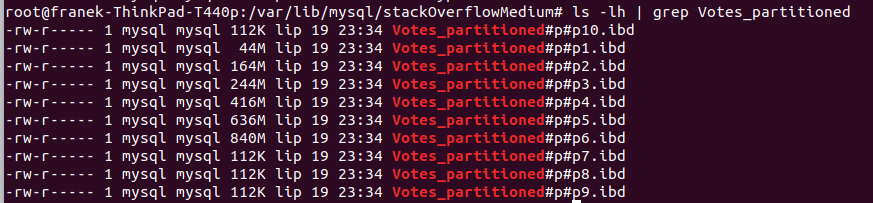
\includegraphics[scale = 0.43]{votes_partitioned_files.png}
	\label{fig:votes_partitioned_files}
\end{figure}

\subsubsection{List partitioning}
Ten typ partycjonowania jest bardzo podobny co do zasady do poprzedniego; rozdział dokonywany jest na podstawie przynależności do pewnego zbioru danych. Przykładowo mieszkańcy Polski i Niemiec trafiają do partycji p1, mieszkańcy Włoch, Francji i Hiszpani do partycji p2, natomiast mieszkańcy Wielkiej Brytani i Irlandi do partycji p3. Z racji anologicznej zasady działania, ta metoda sprawdza się dobrze w dokładnie takich samych przypadkach, jak \textit{range partitioning}.
\subsubsection{Key partitioning}
Bardzo podobne do poprzedniej metody, natomiast funkcja mieszająca wybierana jest przez serwer MySQL. Przykładowo dla \textit{NDB Cluster} używana jest funkcja MD5.
\subsubsection{Hash partitioning}
Partycjonowanie dokonywane jest na podstawie wyniku pewnej funkcji mieszającej (\textit{hash function}) podanej przez użytkownika.

\subsection{Przypadki użycia}
Załóżmy teraz, że chcemy pobrać liczbę ocen ocen ''Spam'' w roku 2013. Pole \textit{CreationDate} nie jest indeksowane. Przygotowałem następujące zapytanie dla dwóch tabel przygotowanych wcześniej:
\begin{spverbatim}
	SELECT count(id) FROM Votes_partitioned v WHERE v.VoteTypeId = 12 AND v.CreationDate BETWEEN '2013-01-01' AND '2013-12-31'; 
	SELECT count(id) FROM Votes v WHERE v.VoteTypeId = 12 AND v.CreationDate BETWEEN '2013-01-01' AND '2013-12-31';
\end{spverbatim}
Porównajmy najpierw wyniki polecenia EXPLAIN dla obu zapytań. Na rysunku ~\ref{fig:explain_range_partition1} przedstawiono wynik dla tabeli partycjonowanej, a na ~\ref{fig:explain_without_rage_partition1} dla niepartycjonowanej. Jak widzimy już na etapie optymalizacji serwer wybrana została partycja w której wyszukiwane będą rekordy. Z tego powodu liczba rekordów do przeszukania jest niemal trzykrotnie mniejsza dla tabeli \textit{Votes\textunderscore partitioned}. Czasy wykonania zapytania dla obu tabel to kolejno: 10.03 sekund dla tabeli partycjonowanej i 17.58 dla niepartycjonowanej.
\begin{figure}
	\caption{}
	\centering
	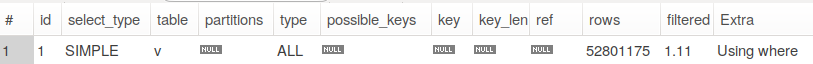
\includegraphics[scale = 0.43]{explain_without_rage_partition1.png}
	\label{fig:explain_without_rage_partition1}
\end{figure}
\begin{figure}
	\caption{}
	\centering
	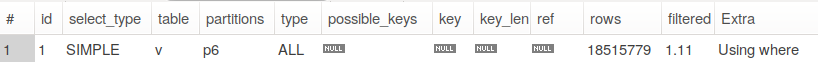
\includegraphics[scale = 0.43]{explain_range_partition1.png}
	\label{fig:explain_range_partition1}
\end{figure}

Kolejnym przypadkiem użycia jest usuwanie dużej ilości danych. Załóżmy przykładowo, że chcemy usunąć wszystkie oceny starsze niż 1 stycznia 2009, czyli de facto dane z partycji \textit{p1}. Przygotowaliśmy dwa następujące zapytania:
\begin{spverbatim}
	SET SQL_SAFE_UPDATES = 0;
	DELETE FROM Votes v WHERE v.CreationDate < '2009-01-01';
	ALTER TABLE Votes_partitioned DROP partition p1;
\end{spverbatim}
Usuwanie danych z tabeli \textit{Votes} trwało 60.903 sekundy, natomiast drugie jedynie 0.073 sekundy. To pokazuje, że szczególnie dla bardzo dużych rozmiarów danych uswanie całych partycji jest zdecydowanie szybsze niż usuwanie wielu pojedynczych wierszy.

Zasadniczo partycjonowanie powinno być jednym z ostatnich etapów optymalizacji i być wykonywane głównie dla tabel z ogromnymi ilościami, ponieważ szereg ograniczeń wynikających z użycia tabel partycjonowanych, jak i dodatkowy nakłada pracy wynikający z konieczności utrzymywania partycji (przykładowo dodawanie kolejnych partycji w kolejnych latach, jeżeli data jest używana do partycjonowania) mogą nie być warte pewnego wzrostu wydajności, który możemy uzyskać również stosując pozostałe metody optymalizacji.

